\documentclass[a4paper]{article}
\usepackage[english]{babel}
\usepackage[utf8x]{inputenc}
\usepackage[T1]{fontenc}
\usepackage{listings}
\usepackage[a4paper,top=2cm,bottom=2cm,left=2cm,right=2cm,marginparwidth=1.75cm]{geometry}
\usepackage{amsmath}
\usepackage{graphicx}
\usepackage[colorinlistoftodos]{todonotes}
\usepackage[colorlinks=true, allcolors=blue]{hyperref}
\setlength\parindent{0pt} % indent
\graphicspath{ {./} }

% my commands:
\newcommand{\n}{\newline}
\newcommand{\tab}{\hspace{1cm}}

\begin{document}
\vspace{-4cm}
{\fontfamily{pbk}\fontsize{12}{15}\selectfont \hspace{-0.5cm}\text{3. domácí úkol | Vilém Zouhar}}


\section{}
Vyřešeno na papíře se zadáním. ($ a_n = -1 + 3n + 2^n$)

\section{}
Nejprve ukážeme, že počet správných uspořádání u stolu je stejný jako počet správných uzávorkování a pak že počet správných uzávorkování je stejný jako počet binárních stromů.

\subsection{}
\textbf{Tvrzení:} Počet správných uspořádání u stolu velikosti $2n$ je stejný jako počet správných uzávorkování délky $2n$. Dobré uspořádání u stolu je takové, že neexistuje čtveřice $(a, b, c, d)$ sedící u stolu v tomto pořadí, která si chce podat ruce: $(a, c), (b, d)$.
\vspace{0.4cm}

\textbf{Příklad:} \n \vspace{0.5cm} \n

\text{}\hspace{2.6cm}\texttt{( ( () ) ) ()}  \hspace{1.6cm} $\Leftrightarrow$  \n
\text{}\hspace{2.6cm}\texttt{1 2 34 5 6 78} \n
\vspace{-3.3cm}
\begin{figure}[h]
	\centering \hspace{4cm}
	 \includegraphics[width=3.5cm]{seating}
\end{figure}

\vspace{0.3cm}
\textbf{Důkaz:}
Nejprve ukážeme, že všechna uzávorkování tvoří správné uspořádání u stolu. $p_o(i)$ := počet otevíracích závorek v řetězci od 1 po i (včetně), $p_u(i)$ := počet uzavíracích závorek v řetězci od 1 po i (včetně). Správné uzávorkování (v řetězci délky $2n$) je takové, pro které:
\begin{align*}
	& \forall i: p_u(i) \le p_o(i) \tab \wedge \tab p_u(2n) = p_o(2n)
\end{align*}
V každém bodě se tedy neuzavírá víc závorek než těch, které jsme otevřeli. Proto nikdo nikdy nepodá ruce křížem (neexistuje závadná čtveřice), neboť na to by byla potřeba, aby se uzavřela nějaká závorka dřív, než měla (aby v nějakém bodě bylo víc uzavíracích závorek než otevíracích). To ale nastat nemůže. \n
Opačně, když máme zajištěno neexistenci závadné čtveřice. Z toho plyne, že pokud máme seřazené hosty $(a, b, c, d)$ a nahradíme hosta otevírací závorkou, pokud podává ruku někomu novému a zavírací závorkou, pokud podává ruku někomu již objevenému. Nemůže ale nastat, že by bylo víc lidí podávající ruku zpětně než naopak.

Tedy počet uspořádání u stolu je stejný jako počet správných uzávorkování. \n

\textbf{Tvrzení:} Počet správných uzávorkování délky $2n$ je stejný jako počet binárních stromů na $2n$ vrcholech. \n

\textbf{Důkaz:} Vytvoříme zjevnou bijekci pomocí algoritmu. Projdeme řetězec a budeme stavět binární strom. Začneme v kořeni a kdykoliv narazíme na \texttt{(}, vytvoříme v aktuálním vrcholu nového potomka a vnoříme se do něj. Pokud narazíme na \texttt{)}, vrátíme se o jeden stupneň nahoru a vytvoříme pravého potomka, při dalším návratu půjdeme již o úroveň výš. Pokud dostaneme na vstup správné uzávorkování, nemůže se nám stát, že bychom udělali nepovolenou operaci (zpracovávali bychom \texttt{)} v kořeni). To nastat nemůže z první vlastnosti správného uzávorkování. Tedy z každého uzávorkování postavíme binární strom. Pokud ale budeme procházet binární strom v nějakém rozumném smyslu (např. DFS), tak úplně stejným způsobem vytvoříme správné uzávorkování (při DFS se nesnažíme vylézt z kořene a končíme v kořeni).\n
Intuitivnější argument: správné uzávorkování délky $2n$ reprezentuje aritmetické výrazy složené z $n$ binárních operací. Tento výraz můžeme snadno reprezentovat i binárním stromem a naopak. \n
Kažopádně z každého binárního stromu vytvoříme správné uzávorkování a binárních stromů na  $n$ vrcholech (každý uzel stojí dvě závorky) je stejně jako správných uzávorkování délky $2n$.
\n

Z přednášky víme, že binárních stromů je $\frac{1}{1+n} {2n \choose n} $. Tolik je tedy i dobrých uzávorkování a správných rozesazení kolem stolu.
 
\subsection{}
Počet se dá vypočítat i přímo za pomocí nástrojů z přednášky. Záleží nám jen na počtu párů, proto tedy naše funkce ($p$) bude závislá na $n$ (počet párů) a nikoliv na $2n$ (počet lidí), oproti původní funkci $q$. Zjevně totiž platí, že $p_n$ = $q_{2n}$, ale toto bude zjednodušení.

Pokud přidáme dva lidi ($8, 7$) ke stolu, tak:

\begin{figure}[h]
	\centering \hspace{4cm}
	\includegraphics[height=3.5cm]{seating_2}
\end{figure}
\hspace{3cm}\textbf{A}\hspace{3.2cm}\textbf{B}\hspace{3.2cm}\textbf{C}\hspace{3.2cm}\textbf{D}

\renewcommand{\theenumi}{\Alph{enumi}}
\begin{enumerate}
	\item podají si ruce $8, 7$ a ostatní možnostmi jak předtím ($p_1\cdot p_3$)
	\item podají si ruce $8, 5$ a ostatní možnostmi jak předtím ($p_1\cdot p_1 \cdot p_2$)
	\item podají si ruce $8, 3$ a ostatní možnostmi jak předtím ($p_1\cdot p_2 \cdot p_1$)
	\item podají si ruce $8, 1$ a ostatní možnostmi jak předtím ($p_1\cdot p_3$)
\end{enumerate}
Celkově $p_1\cdot p_3 + p_1\cdot p_1 \cdot p_2 + p_1\cdot p_2 \cdot p_1 + p_1\cdot p_3 = \sum_{i=0}^{4-1} p_i\cdot p_{4-1-i} = p_4$. To lze zobecnit na: $p_{n} = \sum_{i=0}^{n-1} p_i\cdot p_{n-1-i}$, pro přehlednost $p_{n+1} = \sum_{i=0}^{n} p_i\cdot p_{n-i}$. Intuitivně ještě $p_0 = p_1 = 1$. Tato posloupnost je zjevně důsledek násobení (konvoluce) dvou stejných vytvořujících funkcí, proto musí platit:
\begin{align*}
	& p(x) = x\cdot p^2(x) + 1 \Rightarrow p(x) = \frac{1\pm \sqrt{1- 4x}}{2x}\\
	& \frac{1 - \sqrt{1- 4x}}{2x} \text{ konverguje pro $x$ v okolí nuly, což se nám hodí a proto tento kořen použijeme} \\
	& \text{za pomocí zobecněné binomické věty: } \sqrt{1- 4x} = \sum_{i=0}^\infty { \frac{1}{2} \choose i} (-4x)^i \\
	& \text{nyní bychom normálně hledali koeficient u $x^i$, ale v předpisu dělíme tuto řadu $-2x$, proto nás zajímá $x^{i+1}$} \\
	&  { \frac{1}{2} \choose i+1} (-4)^{i+1} = \frac{\frac{1}{2}\cdot \frac{-1}{2}\cdot \frac{-3}{2}\cdot \dots \frac{1-2i}{2} }{(i+1)!} (-1)^{i+1} 2^{2i+2} = \frac{1 \cdot 1 \cdot 3 \cdot 5 \cdot \dots \cdot (2i-1)}{(i+1)!} (-1)^1 \cdot 2^{i+1} = \\
	& -\frac{1 \cdot 1 \cdot 3 \cdot 5 \cdot \dots \cdot (2i-1) \cdot i!}{(i+1)! \cdot i!} 2^{i+1} = \text{(vynásobíme každý člen faktoriálu v čitateli dvojkou) } = -2\cdot \frac{(2i)!}{(i+1)\cdot i! \cdot i!} = \\
	& -\frac{2}{i+1} { {2i} \choose i}, \text{ (nesmíme zapomenout na dělení $-2$ z původního výrazu) } \rightarrow p_n = \frac{1}{n+1} { {2n} \choose n}
\end{align*}
Dospěli jsme ke stejnému závěru jako v minulém postupu.
\pagebreak

\section{}
\subsection{}
\begin{align*}
	& A(x) + x^{n/2}(C(x)-A(x)-B(x)) + x^nB(x) = \\
	& D_P(x)D_Q(x) + x^{n/2} ( D_P(x)D_Q(x) + H_P(x)H_Q(x) + H_P(x)D_Q(x)+D_P(x)H_Q(x) -  D_P(x)D_Q(x) \\
	& \hspace{10cm} - H_P(x)H_Q(x)) + x^nH_P(x)H_Q(x) = \\
	& D_P(x)D_Q(x) + x^{n/2} (H_P(x)H_Q(x) + H_P(x)D_Q(x)) + x^nH_P(x)H_Q(x) =\\
	& (D_P(x) + x^{n/2}H_P(x))(D_Q(x) + x^{n/2}H_Q(x)) =  P(x) Q(x)
\end{align*}
Ověřeno.

\subsection{}
\begin{align*}
	& \text{Počet násobení pro výpočty jednotlivých pomocných polynomů: } \\
	& A \mapsto 1 \cdot N(n/2), B \mapsto 1 \cdot N(n/2), C \mapsto 1 \cdot  N(n/2), PQ \mapsto 3\cdot N(n/2) \\
	& \Rightarrow N(n) \le 3 N(n/2) \text{ (některá násobení se nám můžou opakovat, proto horní odhad)}
\end{align*}

\subsection{}
\begin{align*}
	& \text{Pro zjednodušení zavedeme funkci } T: \mathbf{N} \mapsto \mathbf{N}: T(i) := N(2^i) \le 3 N(2^i/2) = 3T(i-1) \\
	& \Rightarrow T(i) \le 3 T(i-1) \Rightarrow T(i) \le 3^i \\
	& \big( n = 2^i \rightarrow i = \log_2(n) \big) \Rightarrow N(2^{\log_2(n)}) = N(n) \le 3^{\log_2(n)} \\
	& N(n) \le (2^{log_2(3)})^{\log_2(n)} = n^{\log_2(3)} \Rightarrow N(n) \le n^{\log_2(3)} \\
\end{align*}

\subsection{}
\begin{align*}
	& (2^{10})^2 = 2^{20} >> 2^{10 \log_2(3)} = (2^{10})^{\log_2(3)} \hspace{0.7cm} (\log_2(3) \approx 1.58) \\
	& \frac{2^{20}}{2^{10 \log_2(3)}} \approx 2^{4.15} \approx 17 \Rightarrow \text{ alternativní metoda je zhruba $17$x úspornější}
\end{align*}

\end{document}
